\chapter{Validierung}
Mit Hilfe der Validierung soll festgestellt werden, ob die gestellten Anforderungen erreicht wurden.
Besonders interessant sind im Falle des Paper-Trackers zum einen die Genauigkeit, mit der ein Tracker lokalisiert werden
kann und zum anderen, wie gut das Gesamtsystem miteinander funktioniert und bedienbar ist.
Auch das Setup eines neuen Paper-Tracker-Systems soll dabei mit berücksichtigt werden.

\section{Genauigkeitsmessung des Trackings}

\subsection{Beschreibung}
Bei der Validierung der Genauigkeit des Trackings soll in mehreren Versuchen ermittelt werden, wie genau die Position
eines Dokuments mit Hilfe der Technik des Paper-Trackers bestimmt werden kann.
Das zu erreichende Ziel, um die gestellten Anforderungen zu erzielen, ist eine raumgenaue Ortung (\ref*{fa:tracking}).

\subsection{Durchführung}
Um die Genauigkeit des Systems zu messen, wird eine Reihe an Versuchen durchgeführt, die alle einem gemeinsamen Muster folgen:
\begin{enumerate}
	\item Zurücksetzen des kompletten Systems
	\item Hinzufügen des Trackers
	\item Hinzufügen der in diesem Versuch verwendeten Räume
	\item Einlernen der Räume in beliebiger Reihenfolge
	\item Räume in gegebener Tracking Reihenfolge abgehen
	\begin{enumerate}
		\item Für einige Sekunden im Raum verbleiben
		\item Im Abstand von einigen Sekunden an verschiedenen Stellen im Raum die Position des Trackers bestimmen
	\end{enumerate}
\end{enumerate}
Ein Versuch gilt als erfolgreich, wenn alle Räume in gegebener Reihenfolge richtig erkannt werden bzw. auch in einem
Negativ-Test nicht erkannt werden.

Die auszuführenden Versuche sind sortiert von \enquote{einfachen} zu \enquote{schwierigen} Situationen.
Als einfach zählt zum Beispiel ein Versuch mit nur einem Raum und zu schwierig, wenn als Raum nur eine
Raumhälfte verwendet wird.
Folgendes sind die auszuführenden Versuche:
\begin{enumerate}[label=\textbf{TS-\arabic*}]
	\item \label{ts:gleicher-raum} Ein Raum wird eingelernt und in diesem getrackt
	\item \label{ts:entfernter-raum} Ein Raum wird eingelernt und in einem entfernten Raum getrackt
	\item \label{ts:angrenzender-raum} Ein Raum wird eingelernt und in einem angrenzenden Raum getrackt
	\item \label{ts:zwei-nacheinander} Zwei entfernte Räume werden eingelernt und in selbiger Reihenfolge getrackt
	\item \label{ts:zwei-angrenzende-nacheinander} Zwei angrenzende Räume werden eingelernt und in selbiger Reihenfolge getrackt
	\item \label{ts:raumhälften} Ein Raum wird in zwei Raumhälften geteilt, welche als Räume getrackt werden und in selbiger Reihenfolge getrackt
\end{enumerate}

Zu den Ergebnissen der Versuche selbst muss auch das Umfeld der Versuche angegeben werden.
Dies ist das Gebäude, in dem der Versuch stattgefunden hat, eine ungefähre Raumgröße, die Entfernung der Räume zueinander
und die Struktur des für das Tracking verwendeten \gls{WLAN}-Netzes.

\subsection{Ergebnisse}

Die Tests wurden in den Räumlichkeiten der \gls{DHBW} Karlsruhe durchgeführt.
Dabei konnten alle Testszenarien nach Anpassung der Parameter des Tracking-Algorithmus, wie
in \autoref{sec:tracker-lokalisierung} beschrieben, erfolgreich durchlaufen werden.

\subsubsection{Verwendete Räume}

Für die Tests wurden drei Räume verwendet. \emph{Raum 1} und \emph{Raum 2} haben eine Größe von
circa $6m\times10m$, \emph{Raum 3} ist circa $6m\times5m$ groß. Raum 1 und Raum 2 sind dabei direkt
angrenzend, Raum 3 liegt gegenüber von Raum 2. Die beiden Räume werden durch einen ungefähr $1.5m$
breiten Gang voneinander getrennt, wie in \autoref{fig:floorplan} zu sehen ist.

\begin{figure}[htbp]
	\centering
	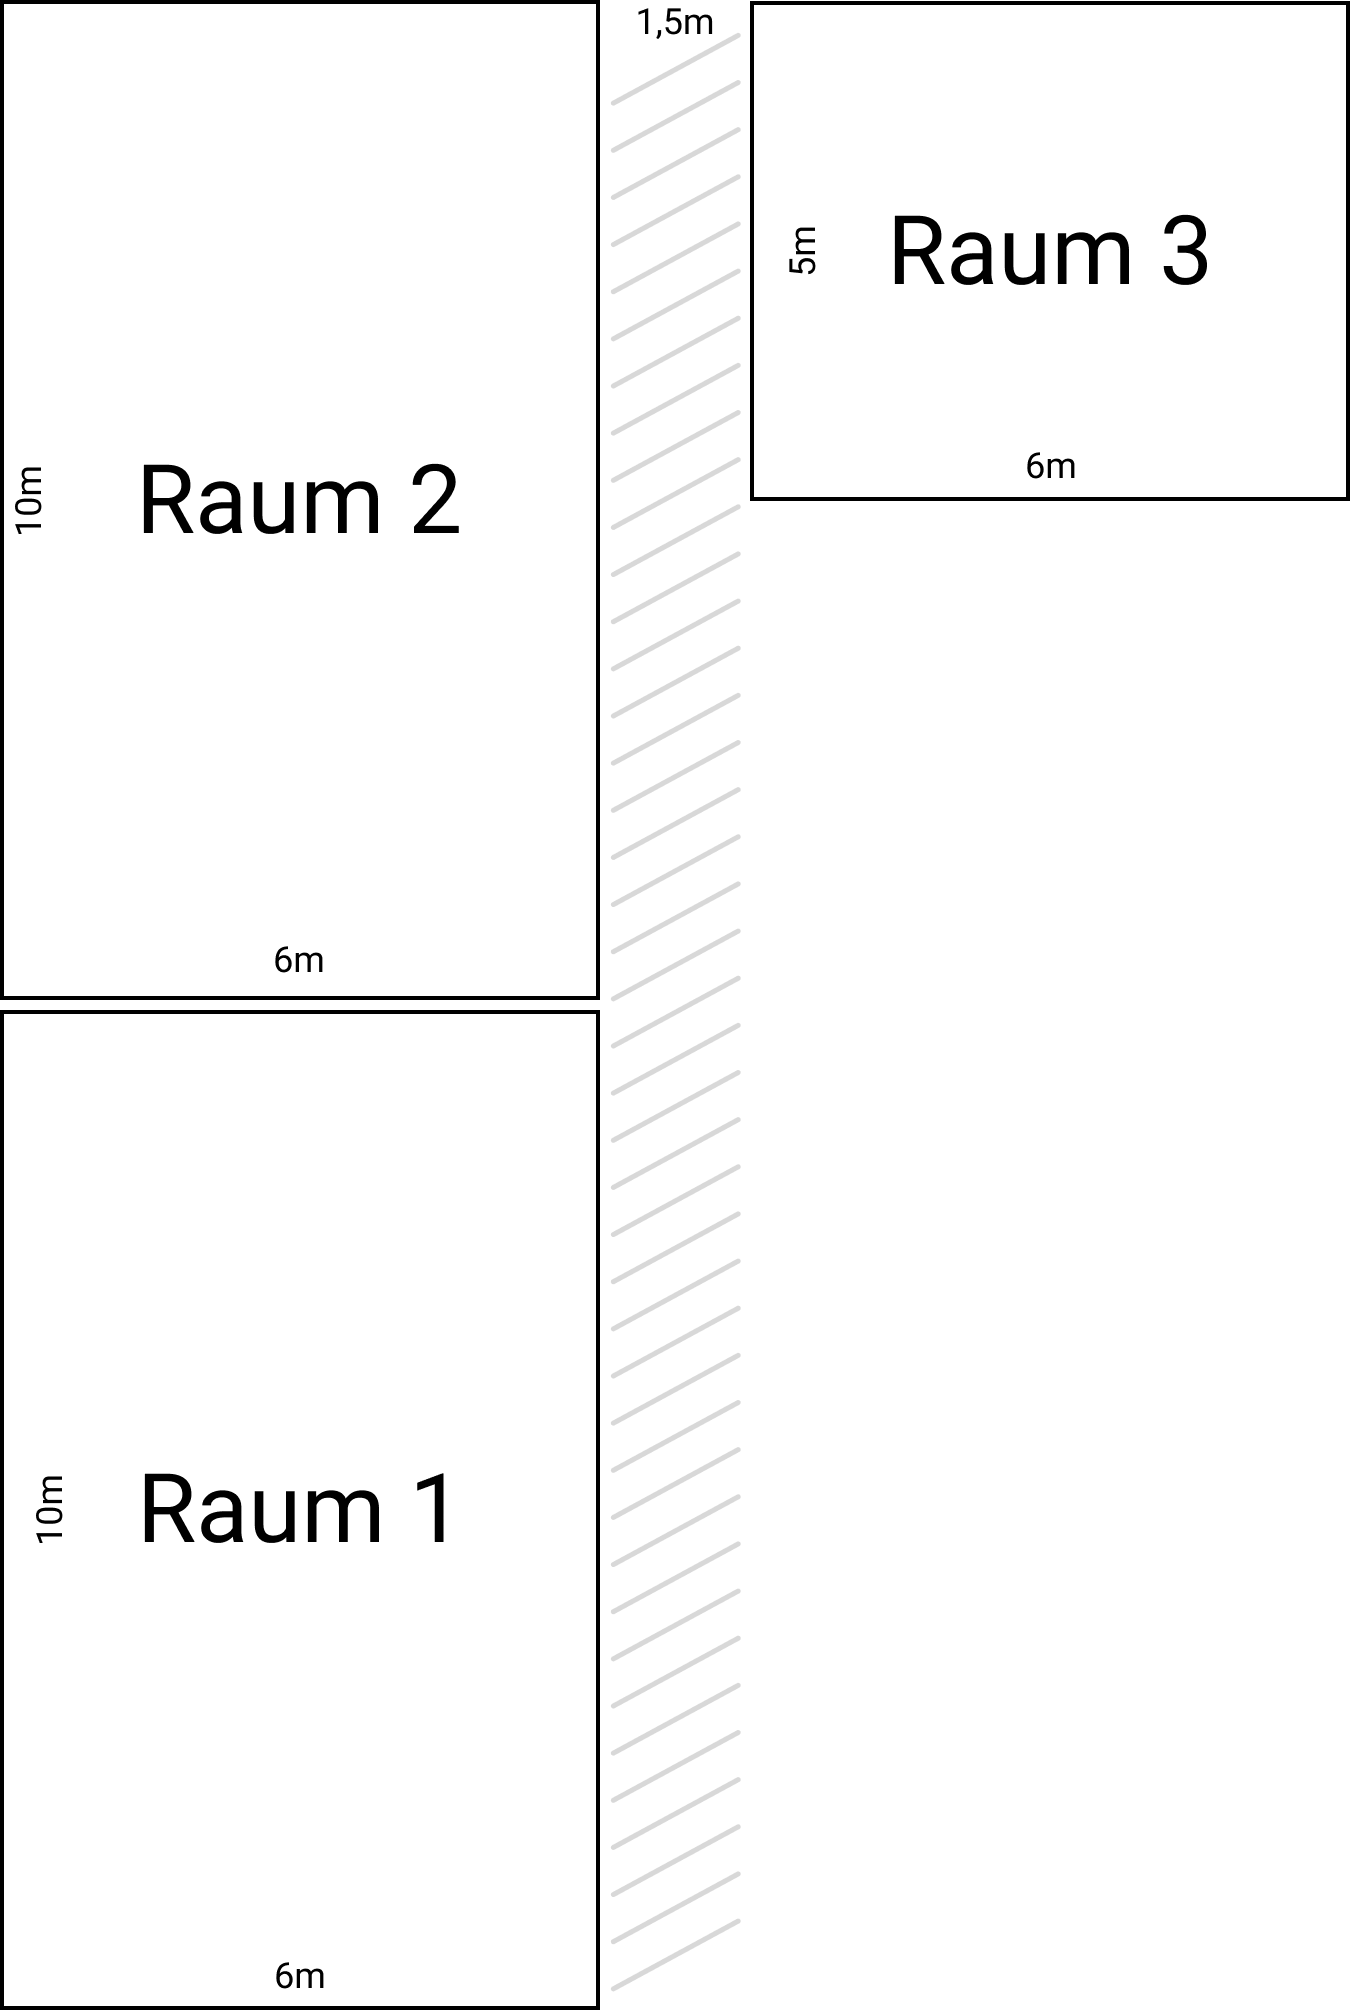
\includegraphics[height=.6\textheight]{images/floor-plan.png}
	\caption{Raumplan für die Testumgebung}
	\label{fig:floorplan}
\end{figure}

\FloatBarrier

\subsubsection{Testszenario 1, 2 und 3}

Für das erste Szenario (\ref{ts:gleicher-raum}) wurde Raum 1 in das System eingelernt. Im Anschluss
wurde erfolgreich überprüft, dass das System den Tracker diesem Raum zuordnet, wenn er lokalisiert
wird.

Im Raum 1 wurden $30$ \glspl{AP} in der \gls{WLAN}-Umgebung gemessen. Ein Ausschnitt aus den
entsprechenden Daten ist in \autoref{tab:wlan-umgebung-raum1} zu sehen.

\begin{table}[htbp]
	\def\arraystretch{1.1}
	\centering
	\begin{tabular}{l c c c c c c}
		\gls{BSSID}	 & Minimum & Maximum & Median & Mittel & 1. Quartil & 3. Quartil \\ \hline
		\texttt{7C:95:F3:72:59:52} & $-74$     & $-73$     & $-73.0$  & $-73.3$  & $-74.0$ & $-73.0$ \\
		\texttt{70:6D:15:F6:5E:44} & $-83$     & $-81$     & $-82.0$  & $-82.0$  & $-83.0$ & $-81.0$ \\
		\texttt{0C:75:BD:BC:85:24} & $-87$     & $-83$     & $-83.0$  & $-84.3$  & $-87.0$ & $-83.0$ \\
		\texttt{7C:95:F3:72:17:B0} & $-89$     & $-88$     & $-88.5$  & $-88.5$  & $-89.0$ & $-88.0$ \\
		\texttt{00:EA:BD:76:21:23} & $-65$     & $-64$     & $-64.0$  & $-64.3$  & $-65.0$ & $-64.0$ \\
		\texttt{70:6D:15:E4:6F:00} & $-74$     & $-72$     & $-73.0$  & $-73.0$  & $-74.0$ & $-72.0$ \\
		\texttt{70:6D:15:E4:6F:05} & $-73$     & $-72$     & $-73.0$  & $-72.6$  & $-73.0$ & $-72.0$ \\
		\texttt{DC:A5:F4:8D:DC:D3} & $-88$     & $-86$     & $-88.0$  & $-87.3$  & $-88.0$ & $-86.0$ \\
		\texttt{00:EA:BD:76:21:20} & $-62$     & $-60$     & $-62.0$  & $-61.36$ & $-62.0$ & $-60.0$ \\
		\texttt{70:6D:15:E4:6F:02} & $-73$     & $-72$     & $-73.0$  & $-72.6$  & $-73.0$ & $-72.0$ \\
	\end{tabular}
	\caption{Ausschnitt aus der \gls{WLAN}-Umgebung von Raum 1}
	\label{tab:wlan-umgebung-raum1}
\end{table}

Für den ersten Negativtest wurde der Tracker in Raum 3 gelegt. Hierbei wurde der Tracker, wie
erwartet, nicht mehr Raum 1 zugewiesen, sodass auch dieser Test bestanden wurde. Auch als der
Tracker für den zweiten Negativtest (\ref{ts:angrenzender-raum}) in Raum 2 gelegt wurde, erkannte
das System korrekt, dass er nicht in Raum 1 liegt, da der vorher eingetragene Score-Schwellwert
nicht erreicht wurde.

\subsubsection{Testszenario 4}

Im Anschluss an den ersten Test wurde der Raum 3 eingelernt, um, wie in \ref{ts:zwei-nacheinander}
beschrieben, in einem \enquote{entfernten} Raum zu tracken. Ziel dieses Tests ist es, zu überprüfen,
ob der korrekte Raum ausgewählt wird. Nachdem Raum 3 eingelernt wurde, wurde zunächst hier ein
Tracking-Vorgang gestartet, wobei Raum 3 korrekt lokalisiert wurde. Nun wurde der Tracker in
Raum 1 abgelegt und ein Tracking-Vorgang gestartet. Auch Raum 1 wurde korrekt als aktueller Raum
identifiziert.
Dieser Test zeigt, dass der Tracker zwischen zwei Räumen unterscheiden kann, deren
\gls{WLAN}-Umgebungen sich deutlich unterscheiden.

\subsubsection{Testszenario 5}

Entsprechend \ref{ts:zwei-angrenzende-nacheinander} wurde nun Raum 2 eingelernt und der gleiche Test
wie für \ref{ts:zwei-nacheinander} durchgeführt. Auch hierbei konnten die beiden Räume erfolgreich
unterschieden werden.
Sogar, als der Tracker innerhalb von Raum 2 direkt an die an Raum 1 angrenzende Wand gehalten wurde,
konnte noch der korrekte Raum erkannt werden. Dies zeigt, dass eine Distanz von circa 2 Metern
korrekt gemessen werden kann.

\subsubsection{Testszenario 6}

Für diesen Test wurde Raum 1 in zwei Hälften geteilt, wie in \ref{ts:raumhälften} beschrieben,
sodass er als zwei $6m\times5m$ große Räume angesehen wurde.
Anschließend wurde in beiden Raumhälften ein Lernprozess gestartet und danach jeweils in einer
Raumhälfte ein Tracking-Prozess. Beide Male erkannte das System die richtige Raumhälfte, sodass auch
dieser letzte Test als bestanden anzusehen ist.

\section{Einfaches Setup und Nutzung des Gesamtsystems}
\subsection{Beschreibung}
In dieser Validierung des Projektes soll bewertet werden, wie einfach ein potentieller Nutzer/Betreiber
des Paper-Trackers ein neues System aufsetzen und verwenden kann.
Um dies zu bestimmen, soll eine oder mehrere Testpersonen alleine mit den Informationen aus dem GitHub-Repository, das
den kompletten Code und die Dokumentation beinhaltet, das System aufsetzen und in Betrieb nehmen.
Im Nachhinein wird den Testpersonen einige Fragen zum Prozess gestellt und sie können selbst freies Feedback geben.

\subsection{Durchführung}
Im Folgenden wird beschrieben, wie der Testverlauf für eine Testperson aussieht.
Auch werden die zu erwartenden Schritte, die die Testperson ausführen soll, angegeben.
Die Testpersonen sollten möglichst mit Informatik versiert sein und zuvor schon einmal einen Server mit einer
Applikation in Betrieb genommen haben.
Als Plattform für die App soll, wenn möglich, Android verwendet werden, da dafür bereits fertige Installationsdateien
zur Verfügung stehen.
Für Apple-Geräte ist dies leider nicht möglich.

Zum Start des Tests bekommt die Testperson einige Informationen, was der Paper-Tracker ist, wofür er bestimmt ist
und die Aufgabe, das System in Betrieb zu nehmen.
Weiter bekommt sie als Ressource, wie oben beschrieben, das GitHub-Repository des Paper-Trackers.
Dieses bietet im Detail die folgenden Komponenten:
\begin{itemize}
	\item Source-Code zu der Firmware, dem Flasher, der App und dem Server
	\item Implizit im Server-Code die App und den ausführbaren Flasher
	\item Ein \enquote{Dockerfile} für den Server
	\item Eine \enquote{README}-Datei mit Informationen zum Setup des Servers
	\item Dieses Paper mit weiterführenden Informationen zum kompletten Projekt
\end{itemize}

Mit Hilfe dieser Komponenten werden folgende Schritte von der Testperson erwartet:
\begin{enumerate}
	\item Setup des Servers
	\begin{enumerate}
		\item Lesen der \enquote{README}-Datei
		\item Anpassen der Konfigurationsdatei mit geeigneten Werten
		\item Erstellen des Docker-Images und Start von diesem auf einem Server \hfill \\
			\hspace*{20mm} oder \hfill \\
			Lokal den Code kompilieren, kopieren der ausführbaren Datei auf den Server, Starten der Datei
	\end{enumerate}
	\item Aufrufen der Download Seite des Servers
	\item Download der Android App und Installation
	\item Durcharbeiten des Tutorials innerhalb der App inklusive des Flashen eines Trackers
\end{enumerate}

\subsection{Ergebnisse}

\section{Gesamtergebnis der Validierung}
